\newpage
\section{Wearable \& Handheld} \label{sec:hauptteil_android}

\subsection{Android (Standard)}
Das Android-Betriebsystem erfreut sich weltweit größter Beliebtheit. Android ist mit über 75\% auf dem Markt das meist verbreitete Mobil-Betriebsystem für Smartphones und Tablets. Ein großer Vorteil des mobilen Betriebssystems ist die Möglichkeit, die Funktionalität durch Installation zusätzlicher Anwendungen (Apps) zu erweitern.
\\[0.5cm]
Erstellt werden Apps i.d.R. mit Hilfe des Android Frameworks in der Programmiersprache Java. Das Android Framework passt in die Kategorie der modernen Gui-Frameworks, da die Programmlogik strikt von den Definitionen für das Layout getrennt ist. Das Layout wird durch Dateien mit XML-Struktur festgelegt und kann so unabhängig vom Code angepasst werden.

\subsection{Android Wear}
Android Wear als noch recht neues Betriebssystem stellt eine ressourcenschonende Version des Standard-Android-Betriebssystems für Wearables (Smartwatches, Armbänder, etc.) dar. Die Wearables bringen in den meisten Fällen Sensoren für Fitness-Tracking (z.B. Pulsmesser, und Schrittzähler) mit, die durch die Android API bereits unterstützt werden. Das Wearable-Gerät kann zwar selbstständig agieren, ist jedoch ohne entsprechende Hardware zur Nutzung von Internet, W-Lan oder anderen Ressourcen auf ein gekoppeltes Handheld-Gerät angewiesen. Auch Hersteller Google betont, dass das Betriebsystem grundlegend zur Kopplung mit einem Smartphone bzw. Tablet (Im folgenden allgemein: Handheld) ausgelegt ist. Notifications vom Handheld, werden beispielsweise bequem auf das Wearable-Gerät weitergeleitet, während in die andere Richtung Spracheingaben auf dem Wearable-Gerät interpretiert und zum Handheld-Gerät zur weiteren Verarbeitung übermittelt werden können. Die Kommunikation findet dabei i.d.R. über eine spezielle Wearable-Bluetooth-API statt.
\\[0.5cm]
Die Design-Prinzipien, die grundlegend auf den Entwicklerseiten von Android Wear empfohlen werden, unterstreichen ebenfalls die enge Verbundenheit zum Handheld-Gerät. So sollen rechen- bzw. zeitintensive Tasks auf das leistungsfähigere Handheld-gerät ausgelagert werden und Konfigurationen für Wearable-Apps weitesgehend auf dem Handheld-Gerät vorgenommen werden. So bietet es sich an, für eine Wearable-App gleich eine zugehörige Handheld-App mitzuliefern. Die Installation einer Wearable-App erfolgt dabei auch über das Handheld-Gerät: Eine APK-Installations-Datei kann mehrere Apps für verschiedene Geräte enthalten, die dann automatisch verteilt werden. Apps für Android Wear werden unter den gleichen Bedingungen erstellt, wie Apps für das Standard-Android-Betriebssystem. Zusätzlich unterstützt Android Wear sowohl runde und quadratische Display-Typen, was bei der Gestaltung des Layouts zu beachten ist.

\subsection{Anforderungen}
Im vorliegenden Projekt soll ein Wearable-Gerät, das über einen Pulsmesser- und Schrittzähler-Sensor verfügt, die jeweiligen Werte über einen begrenzten Zeitraum auslesen und temporär verwalten. Dieser Vorgang wird folgend als Messung bezeichnet. Dabei wird zwischen Aktivitäts- und Ruhemessung entschieden. Ersteres soll die Daten solange aufzeichnen, bis die Messung vom Benutzer beendet wird und Letzteres soll festgelegt eine einmütige Messung durchführen und den Median-Wert bilden. Die Auswahl über die Art der Messung soll unmittelbar vor der Messung durch den Benutzer stattfinden.
\\[0.5cm]
Im Anschluss an die Messung soll eine Dialog-Abfrage, die Stimmung des Benutzers während der Messung erfassen. Die Messdaten sollen nach Bearbeitung dieses Dialogs ohne zusätzliche Interaktion per Bluetooth zum Handheld-Gerät übertragen werden, sofern dieses Verfügbar ist. Wenn das Handheld-Gerät zu diesem Zeitpunkt nicht zur Verfügung steht, soll der Benutzer die Möglichkeit haben die Messung erneut zu versenden oder zu verwerfen. Eine persistente Speicherung der Messdaten soll dabei auf dem Wearable-Gerät nicht stattfinden. Abbildung \ref{fig:structure_wearable} zeigt die bisher beschriebene Struktur auf.

\bigskip
\begin{figure}[H]
	\visioToPDF{images/structure_wearable.vsd}
	\centering
	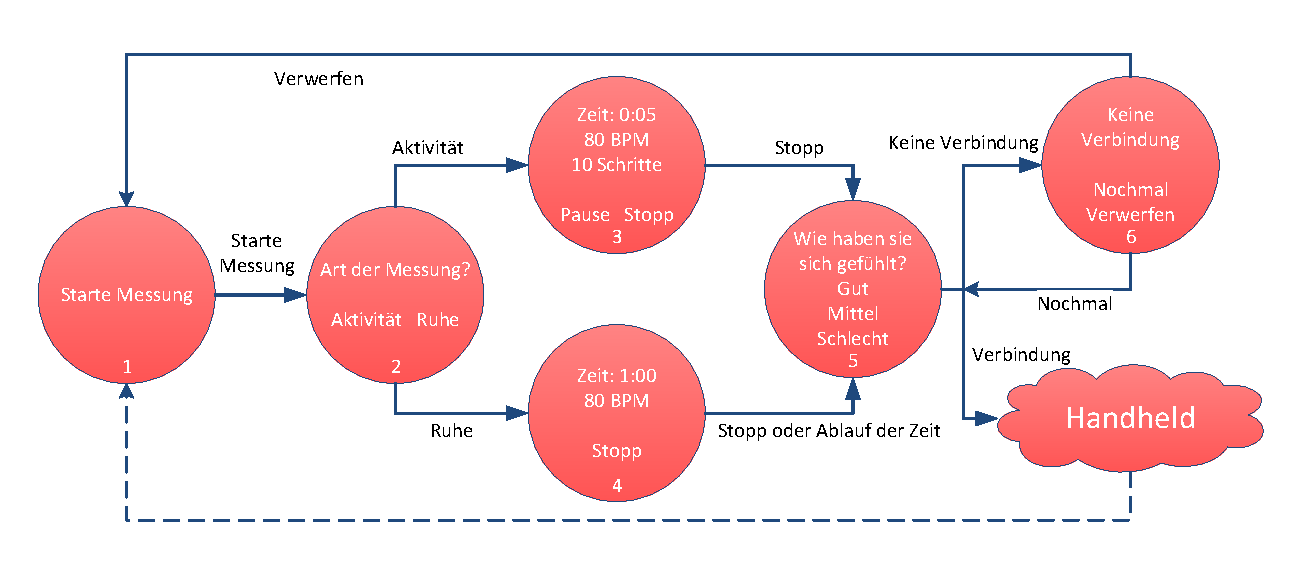
\includegraphics[scale=0.65]{images/structure_wearable.pdf}
	\caption{Struktur der Wearable-App}
	\label{fig:structure_wearable}
\end{figure}
\bigskip

Das Handheld-Gerät soll sich kontinuierlich in Bereitschaft zum Empfang von Messdaten befinden und diese verarbeiten können. Zusätzlich soll die App auf dem Handheld-Gerät über eine grafische Oberfläche zur Konfiguration und zur temporären Verwaltung von Messdaten verfügen. Ein Graph soll die Messungen übersichtlich visualisieren. Eine Bewertung der Daten ist an dieser Stelle nicht erforderlich.
\\[0.5cm] 
Das Handheld-Gerät soll die Messdaten per Bluetooth an ein Bluetooth-fähiges Endgerät weiterversenden können (z.B. PC oder Notebook). Es soll sowohl möglich sein, die Daten automatisch durch den Hintergrund-Dienst versenden zu lassen, als auch die Daten manuell über die grafische Oberfläche zu versenden. Die geplante Struktur der Handheld-App wird in Abbildung \ref{fig:strucure_handheld} dargestellt.

\bigskip
\begin{figure}[H]
	\visioToPDF{images/strucure_handheld.vsd}
	\centering
	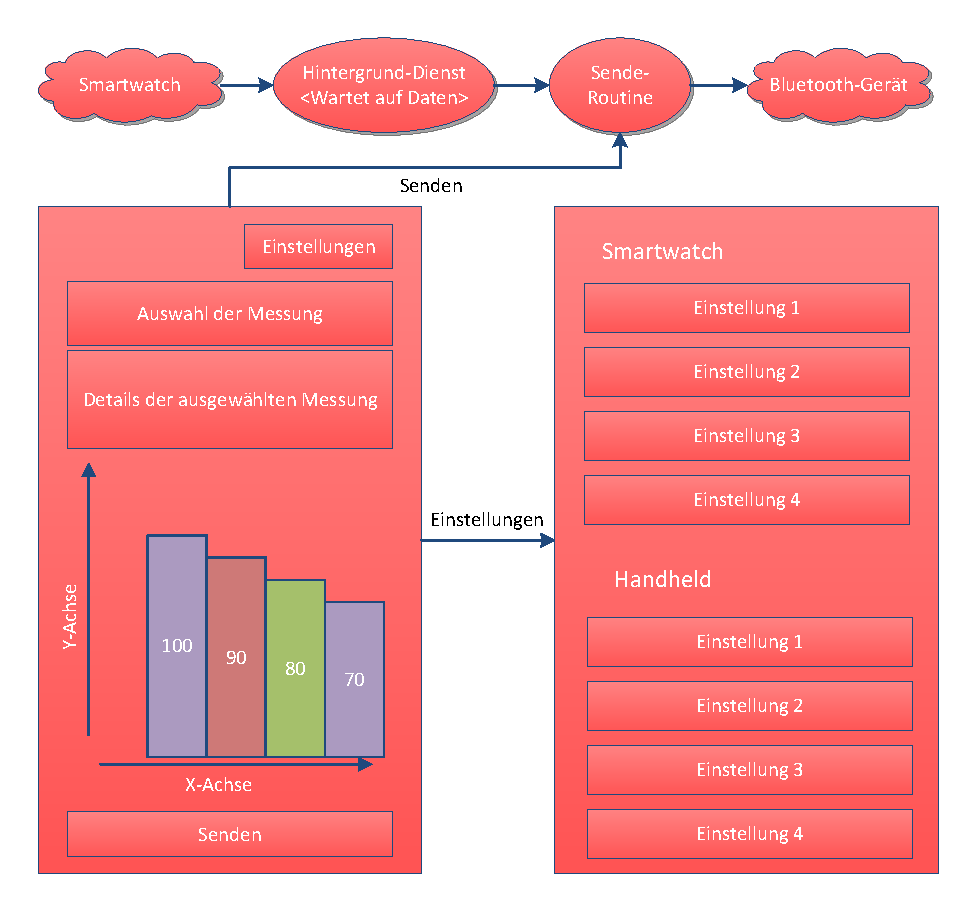
\includegraphics[scale=0.8]{images/strucure_handheld.pdf}
	\caption{Struktur der Handheld-App}
	\label{fig:strucure_handheld}
\end{figure}
\bigskip


\subsection{Vorbereitung}
Im Rahmen des Projektes werden eine Motorola Moto 360 Smartwatch und ein Samsung Galaxy S4 Smartphone als Testgeräte verwendet. Auf der Moto 360 läuft Android Wear in der Version 5.0 und auf dem Galaxy S4 läuft Android in der Version 4.4 (Cyanogenmod 11 Custom-Rom). Die Geräte sind grundsätzlich gekoppelt und die gleichnamige Google App "`Android Wear"' verwaltet auf dem Smartphone (im Hintergrund) die Verbindung zur Smartwatch. Die Entwicklung erfolgt mit Hilfe der Entwicklungsumgebung "`Android Studio"', die ebenfalls von Google veröffentlicht wurde. Dabei kann die Smartphone-App direkt über USB debugged werden, während der Debugging-Vorgang bei der Smartwatch über das gekoppelte Smartphone per Bluetooth gebrückt wird.

\subsection{Einschränkungen}
Bei Verwendung der Bluetooth-Library in der Qt-Framework Anwendung konnten Inkompatibilitäten nicht umgegangen werden (Näheres im Abschnitt QT Framework Anwendung). Da das Software-Paket sich letztlich an den gewöhnlichen Heimanwender richtet, ist grundsätzlich ein Heimnetzwerk mit Router und verbundenen Endgeräten zu erwarten. Aus diesen Gründen soll die von der Handheld-App ausgehende Verbindung als TCP/IP Verbindung implementiert werden. Dabei soll ein UDP-Broadcast verwendet werden, um die Handheld-App im Netzwerk bekannt zu machen. Dadurch soll der Anwender Konfigurationsaufwand einsparen. Alternativ soll aber auch eine feste Adressierung möglich sein.

\subsection{Implementierung}
TODO
\subsubsection{Wearable-App}
TODO
\subsubsection{Handheld-App}
TODO

\subsection{Tests}
Es werden unterschiedliche Testfälle hinsichtlich Fehlerverhalten bei den vorgesehenen Ausführungsroutinen angefertigt und geprüft. Die Testfälle und deren Ergebnisse werden tabellarisch aufgelistet.
\subsubsection{Wearable-App}
Im Vordergrund steht bei der Wearable-App die ständige Definiertheit des Zustandsautomaten. In folgender Tabelle werden alle Zustände und Folgezustände aufgelistet und verifiziert. 
TODO TABELLE
\subsubsection{Handheld-App}
Die Handheld-App muss in der Rolle des Daten-Vermittlers zwischen Wearable-Gerät und IP-Endgerät die Messdaten zuverlässig und unverändert weiterleiten. Die korrekte Darstellung von Messdaten ist ebenfalls ein Testkriterium. Außerdem wird die Anwendung und Übertragung von Einstellungen geprüft. Die nachstehende Tabelle zeigt die Testkriterien auf.
TODO TABELLE

%\lstset{language=Java}
%\begin{lstlisting}[caption=Listing, label=lst:Listing]
%\end{lstlisting}

%\begin{shaded}
%Text in Textbox
%\end{shaded}

%\ref{sec:hauptteil}
%\cite{audio_architecture}